%*******************************************************************
%   Project Name: BracU Thesis Template
%   Prepared by: Ayesha Abed Library, Brac University
%   
%   "Predicting a T20 Cricket Match Result While The Match is in Progress", this thesis was 
%   submitted to BracU on 23 August, 2015 by Fahad Munir, Md. Kamrul Hasan, Sakib Ahmed, Sultan Md. Quraish
%   Authors have given full consent to use their thesis as a sample to develop a Thesis Template using LaTex 
%   PLEASE KEEP ALL FILES IN THEIR DESIGNATED FOLDERS
%*******************************************************************
% Project Structure:
% appendix: Contains “appendix.txt” files.
% bibliography: Contains “references.bib” file.
% chapters: Contains “chapter.txt” files. For every chapter, create separate “chapter_[1,2,3..].txt” files.
% core: This folder will contain following files:
%     declaration.txt
%     approval.txt
%     ethics_statement.txt
%     abstract.txt
%     dedication.txt
%     acknowledgement.txt
%     titlepage.txt
% images:Contains all images files. 
% main.txt
%     This is the main.txt file. All the packages and environment variable are declared in main.txt. All others .txt files are referred from this file.
%
% If you have any questions or concerns about the latex template, please feel free to visit Ayesha Abed Library.
%*******************************************************************

\documentclass[Times,12pt,oneside,openany,print,index]{report}
\usepackage[a4paper,width=150mm,top=25mm,bottom=25mm]{geometry}
\usepackage[english]{babel}
\usepackage[utf8]{inputenc}
\usepackage{csquotes} % Provides advanced facilities for in-line and display quotations
\usepackage{amsmath} % TO use mathematical equations 
\pagestyle{plain} % Just a plain page number. For more http://www.emerson.emory.edu/services/latex/latex_129.html

\usepackage{graphicx} % to use the graphicx package
\graphicspath{/images} % Path to Image files 
\usepackage{caption} % To use caption with figure and images
\usepackage{array} % The array environment is used to make a table of information, with column alignment (left, center, or right) and optional vertical lines separating the columns

\usepackage[nottoc]{tocbibind} % The tocbibind package can be used to add the ToC and/or bibliography and/or the index etc., to the Table of Contents listing

\usepackage[normalem]{ulem} % The ulem package provides various types of underlining that can stretch between words and be broken across lines.

\usepackage{hyperref} % Provides LaTeX the ability to create hyperlinks within the document.
\hypersetup{
    colorlinks=true,
    linkcolor=black,
    filecolor=magenta,      
    urlcolor=black,
    citecolor=black,
}
\urlstyle{same}

\setlength{\parindent}{0em} % To control Indentation of paragraphs 

\usepackage{nomencl} % The nomenclature package can be used to generate and format a nomenclature using MakeIndex.
\renewcommand{\nompreamble}{The next list describes several symbols \& abbreviation that will be later used within the body of the document}
\makenomenclature

\usepackage[backend=biber,style=ieee,sorting=ynt]{biblatex} % for more plz click https://www.overleaf.com/learn/latex/Biblatex_citation_styles
\addbibresource{bibliography/references.bib} % Imports bibliography file

\let\cleardoublepage=\clearpage % removes unwanted doublepages

\begin{document}

\thispagestyle{empty} % removes page number from title page
\begin{titlepage}
\renewcommand*{\thepage}{Title} % Change page number in PDF

    \begin{center} 
        \vspace*{3cm} % For creating Vertical Blank Space
        
        {\fontsize{16pt}{22pt}\selectfont{Predicting a T20 Cricket Match Result While \\
        The Match is in Progress}
        } % "fontsize{font size}{line space}\selectfont{}" command to override font size and line space for the Title
        
        \vspace{1.5cm}
        
        \text{by}
        
        \vspace{0.5cm}
        
        	Student Name\\
	        Student ID\\
	        Student Name\\
	        Student ID\\
	        Student Name\\
	        Student ID\\
	        Student Name\\
	        11000000

        \vspace{1.5cm}
        
        	A thesis submitted to the Department of Computer Science and Engineering\\
            in partial fulfillment of the requirements for the degree of\\
            B.Sc. in Computer Science

        
        \vspace{2.5cm}
        
    		Department of Computer Science and Engineering\\
            Brac University\\
            August 2015
        
        \vspace{3cm}
        
    		\copyright\ 2015. Brac University\\
            All rights reserved.
    
    \end{center}

\end{titlepage} % Add title page
\cleardoublepage

\pagenumbering{roman} % Roman numbers to be use all pages before Chapter 1

%*******************************************************************
% TOC = Table of Contents
% The hyperref makes Title page No. 1 entry in the TOC
% In order to properly link  all section in TOC "phantomsection" command used
%  see below link for details on "addcontentsline"
% http://www.emerson.emory.edu/services/latex/latex_162.html
% "input" command to add files
% "Ethics Statement" & "Dedication" page are Optional; you may omit this two page if you want
% Please do not change the order of listings in TOC
%*******************************************************************
\phantomsection
\addcontentsline{toc}{chapter}{Declaration}
% Following command is used to created grouped signature line for Four Authors
\newcommand*\wildcard[2][6cm]{\vspace{2cm}\parbox{#1}{\hrulefill\par#2}} 

% A "parbox{}{}" is a box whose contents are created in paragraph mode. 
% "hrulefill{} to chance thickness of underline"

\section*{Declaration}

It is hereby declared that

\begin{enumerate} % begin{enumerate} function to create numbered list
  \item The thesis submitted is my/our own original work while completing degree at Brac University.
  \item The thesis does not contain material previously published or written by a third party, except where this is appropriately cited through full and accurate referencing.
  \item The thesis does not contain material which has been accepted, or submitted, for any other degree or diploma at a university or other institution.
  \item We have acknowledged all main sources of help.
\end{enumerate}

\vspace{1cm}
\textbf{Student’s Full Name \& Signature:} % Testbf{} for Bold

\begingroup

    \begin{center}
        \wildcard{\centerline{Student Name} ~\\ \centerline{Student ID}} % "centerline{}" to center line
        \hspace{2cm} % "hspace{}" for Blank Horizontal space
        \wildcard{\centerline{Student Name} ~\\ \centerline{Student ID} }
        \wildcard{\centerline{Student Name} ~\\ \centerline{Student ID} }
        \hspace{2cm}
        \wildcard{\centerline{Student Name} ~\\ \centerline{Student ID} }
    \end{center}

\endgroup


\pagebreak







\phantomsection
\addcontentsline{toc}{chapter}{Approval}
\section*{Approval}

The thesis/project titled “Predicting a T20 Cricket Match Result While The Match is in Progress” submitted by 
\begin{enumerate}
  \item Student Name (Student ID)
  \item Student Name (Student ID)
  \item Student Name (Student ID) 
  \item Student Name (Student ID)
\end{enumerate}

Of Summer, 2015 has been accepted as satisfactory in partial fulfillment of the requirement for the degree of B.Sc. in Computer Science on August 23, 2015. 

\vspace{0.5cm}
\textbf{Examining Committee:}

\vspace{1cm}

Supervisor:\\
(Member)
\begin{center}
    \hspace{7cm} \wildcard{\centerline{Name of Supervisor} ~\\ \centerline{Senior Lecturer}~\\ \centerline{Department}~\\ \centerline{Institution} } \hspace{1cm} 
\end{center}

Program Coordinator:\\
(Member)
\begin{center}
    \hspace{7cm} \wildcard{\centerline{Name of Program Coordinator} ~\\ \centerline{Designation}~\\ \centerline{Department}~\\ \centerline{Brac University} } \hspace{1cm} 
\end{center}

Head of Department:\\
(Chair)
\begin{center}
    \hspace{7cm} \wildcard{\centerline{Name of Head of Department} ~\\ \centerline{Designation}~\\ \centerline{Department of Computer Science and Engineering }~\\ \centerline{Brac University} } \hspace{1cm} 
\end{center}

\pagebreak

\phantomsection
\addcontentsline{toc}{chapter}{Ethics Statement}
\section*{Ethics Statement (Optional)}
This is optional, if you don't have an ethics statement then omit this page
\pagebreak

\phantomsection
\addcontentsline{toc}{chapter}{Abstract}
\section*{Abstract}
Sounds have a wealth of information that enhances our understanding in this unprejudiced world. Every day we face many sounds around us. From this sound we filter all sounds in our brain cell and provide with a result what sounds are fit in which dice. For this not only our brain cells many machines are also available. Working with sound classifications, can improve recommendations in various applications. To work properly these machines, need to know the right way to extract data from it. Digital audio has a lack of structured organizations. So that it brings significant complexity to sound classification work. Keeping that in mind we intended to do research in sound classification. The primary goal of our research is to find which feature fits our model and gives us maximum values that we desire for. All the while we will try to analyze different models to see which work more efficiently. Our plan is to collect speech command dataset from online sources. We intended to use deep learning methods to analyze our data in different features. Those features are MFCC, Mel Spectrogram, Wavelet. For our model we use conventional neural networks (CNN), long short-term memory (LTSM). Also, we will analyze raw data without implementing any features. 




\vspace{1cm}
\textbf{Keywords:}  convolutional neural networks (CNN), LSTM, Deep learning, Mel Frequency Cepstral Coefficient (MFCC), Wavelet. Mel-Spectrogram.
\pagebreak


\phantomsection
\addcontentsline{toc}{chapter}{Dedication}
\section*{Dedication (Optional)}
A dedication is the expression of friendly connection or thanks by the author towards another person. It can occupy one or multiple lines depending on its importance.
You can remove this page if you want.

\pagebreak

\phantomsection
\addcontentsline{toc}{chapter}{Acknowledgment}
\section*{Acknowledgement}
Firstly, all praise to the Great Allah for whom our thesis have been completed without any major interruption.\\
Secondly, to our co-advisor Teacher Name sir for his kind support and advice in our work. He helped us whenever we needed help.\\
Thirdly, Name and the whole judging panel of Conference Name. Though our paper not accepted there, all the reviews they gave helped us a lot in our later works.\\
And finally to our parents without their throughout sup-port it may not be possible. With their kind support and prayer we are now on the verge of our graduation.

\renewcommand{\contentsname}{Table of Contents} % Rename TOC name from Contents to Table of Contents
\cleardoublepage
\phantomsection
\addcontentsline{toc}{chapter}{Table of Contents} % Add Table of Contents in TOC
\tableofcontents % To  generation of the Table of Contents

\listoffigures % To  generation of the List of Figure
\listoftables % To  generation of the Tables of Figure

\printnomenclature % TO  generation of the Nomenclature file
\addcontentsline{toc}{chapter}{Nomenclature}
\cleardoublepage

\pagenumbering{arabic} % To use page number 1,2,3 ..

\chapter{Introduction}
%\section{Introduction}
\section{Audio Classification} 
Audio classification is an expanding field of research with several real-world applications. Recent advances in image classification, where convolutional neural networks are used to classify pictures with high accuracy and at scale, raises the issue of whether similar approaches may be applied to other domains, such as audio classification. Audio classification or sound classification is the process of analyzing audio recordings and categorizing them in a proper way. Basically, audio classification is the task of assigning a label or class to a given audio. It may be used to identify a speaker as well as recognize which command a user is issuing or the mood of a speech. Audio classification can be of multiple types and forms such as-Acoustic event detection, music classification, Natural language classification and environmental sound classification. Despite recent advances in the field of audio classification, teaching a machine to recognize a sound and classify it into several categories is a tedious process. Starting with annotated audio data is the initial step in solving audio categorization challenges. Here are several relevant datasets for various sorts of sounds. These datasets contain a huge number of audio samples, as well as a class label for each sample that indicates what sort of sound it is, depending on the problem we’re attempting to solve. The automated classification of audio is a major challenge. Several authors have proposed methods to categorize incoming audio data based on different techniques throughout the previous decade. The majority of the proposed systems incorporate two phases of processing. The first stage analyzes the incoming waveform and extracts certain features from it. The feature extraction process generally entails a significant amount of data reduction. The second stage performs a classification based on the extracted features. A variety of signal features have been proposed for general audio classification. A second important feature set which is inherited from automatic speech recognizers consists of mel-frequency cepstral coefficients (MFCC). We applied Convolutional Neural Network (CNN) and Recurrent Neural Network (RNN) along with MFCC to improve the work proficiency of our model and tried to make comparisons with other models. CNN has shown to be effective in voice classification. We’ll exhibit how to apply Deep 4 Learning techniques to the classification of audio, specially focusing on the identification of particular sounds.
\section{Problem Statement}
Nowadays in the current world, speech recognition has gained prominence and use with the rise of AI and intelligent assistants, such as Amazon Alexa, Apple Siri, Microsoft Cortana, Google assistant. Speech recognition is the ability of a machine or a program to identify words and phrases in spoken language and convert them to a machine-readable format. Speech recognition has many applications such as voice dialing, call routing, search keywords, simple data entry. Today in the current generation speech recognition is playing a major role in most of the fields such as smartphones, Tv, voice call routing, voice dialing, search keywords, simple data entry. We all know that whenever we call any customer care service there will be a virtual assistant to assist us before we reach the main person to whom we want to talk. The technique used here was Call routing which refers to the procedure of sending voice calls to a specific queue based on predetermined criteria. A call routing system is also known as an automatic call distributor (ACD). Since traditional models of customer service were based on phone support or call support as one of the primary methods of contact between customers and companies for business purposes, the procedure of sending calls to the right agent became very much important. Today, modern agents interact with customers through a variety of channels. In earlier days most of the people use to call by typing the number in the phone but nowadays voice-enabled calling is also available where people use to call anyone through their voice without typing any number in the phone, this has made easier to the people but the problem is if anyone is in such a place where there is more noise and more disturbance then voice-enabled calling may not work correctly as more than two or more voices mixes, where it will be difficult for a system to recognize our voice in such a worst environment. To overcome this best noise elimination technique should be used where it can eliminate noise up to a level. Voice enabled calling is also known as voice dialing which uses speech recognition software. In the present world, it is possible to entry some of the data in excel or word documents using our voice which enables you 6 to do hands-free data entry by dictating the text or numbers that we want to be entered in the current cell and to issue voice commands that allow you to choose menu items, dialog box options, or even toolbar buttons by simply saying their names. This saves our time and work can be done faster compared to typing work. Even for voice data entry speech recognition software has been used. When using Speech Recognition to dictate data entries, we need to keep the microphone close to our mouth and in the same position as you dictate. Depending upon the microphone quality we need to speak normally and in a low but not monotone voice, pausing only when you come to the end of a thought or the data entry for that cell and it takes time for our computer to process our speech, and therefore, depending upon the speed of your processor, it may take some time before your words appear on the Formula bar and in the current cell. This can be improved by training more and more audio data using deep learning or machine learning algorithms. As we know Google Assistant and Microsoft Cortana are widely used nowadays such as searching for information on the internet or it may search for information on the computer such as files, folders, documents, and many other things. All these are done through our voice, whatever we speak, or we tell Google Assistant and Microsoft Cortana it will search and give us a piece of information about what we require. Therefore, Speech recognition is playing a major role in Google assistant, Microsoft Cortana, and Apple Siri. Day by Day the accuracy of converting from speech to text in Google Assistant, Microsoft Cortana, and Apple Siri is increasing. Think of a situation where you want to share your feelings to someone or you want someone to entertain you in your sad times then Amazon Alexa or amazon echo can be used, whenever we speak it will listen to us and give some information like if we tell "Alexa sing a song" it will sing some song for us or if we tell "Alexa tell us some news about today" so Alexa will tell us the news about today, Amazon Alexa is speech recognition device which recognizes our speech and depending upon that it gives some output.
\section{Research Objective }
In our research, we proposed an efficient way to classify audio data of different objects using deep learning methods using neural networks. Here, we aim to prepare a deep learning model that can predict the accuracy of different models through extracting features from the Speech Command dataset. Our prior objective is to determine the wav files so that the devices whose work is based on voice can predict properly and give better results by fulfilling customer requirements. The remaining objective is as follows:
 
•	Organizing Audio library for each class.\\
•	Finding the best performance algorithms which can work more precisely on different scenarios. \\ 
•	By using different feature extraction techniques to analyze music genre identification.\\
•	Finding different audio pattern using deep neural network 


\chapter{Litareture Review}
Better predictive modeling depends on better understanding of the data and attributes selection. We have to choose between some data mining algorithm. We have chosen data mining as it is very much flexible in predictive modeling. Prediction when the game is in progress is a tough ask and it need finding the best attributes that influence the match outcome. Some research was done previously on predictive modeling in sports like Basketball, Baseball along with Test and One Day International cricket.
In basketball, Bhandari et al.\cite{Bhandari1997} developed a knowledge discovery system and data mining framework for National Basketball Association (NBA). It was aimed to discover several interesting patterns in basketball games. This and related system have been used by several basketball teams over the past decades. Such solutions designed for offline usage and no in game effects were taken care of. There has been some recent works (20) about in-game decision making to find how much time remaining in the game without making any prior prediction model.
There were several works done in cricket. Bailey and Clarke\cite{Bailey} and Sankaranarayanan et al.\cite{Sankaranarayanan} used machine learning approach to predict the result of a one day match depending on the previous data and in game data.
Akhtar and Scarf\cite{Akhtar} used multinomial logistic regression in their work on predicting a outcome of a test matches played between two teams.
Choudhury et al.\cite{Choudhury} used Artificial Neural Network to predict result of a multi team one day cricket tournament depending on the past 10 years data. They used training set in order to model the data in neural network. Again there was no in play effects were taken care of.
For baseball, Ganeshapillai and Guttag\cite{Ganeshapillai} developed a prediction model that decides when to change the starting pitcher as the game progresses. It is very much similar to our work-flow, where they used the combination of previous data and in game data to predict a pitchers performance.
Tulabandhula and Rudin\cite{Tulabandhula} were designed a real time prediction and decision system for professional car racing. Model makes the decision of when is the best time for tire change and how many of them. These works supplied a huge encouragement and informative ideas in our research.


\chapter{Prediction Modeling using Decision Tree}
Decision tree algorithm is a very popular way to design a predictive modeling. Decision tree builds classification or regression models in the form of a tree structure. It breaks down a data set into smaller and smaller subsets while at the same time an associated decision tree is incrementally developed. The final result is a tree with decision nodes and leaf nodes. A decision node (e.g., Outlook) has two or more branches (e.g., Runs, Wickets and Run-Rate). Leaf node (e.g., Result) represents a classification or decision. The topmost decision node in a tree which corresponds to the best predictor called root node. Decision trees can handle both categorical and numerical data. Decision tree built on the calculation of Entropy and Information gain.

\section{Entropy Calculation}
Entropy is a measure of unpredictability and uncertainty of a data-set. Entropy is generally considered to determine how disordered a data-set is. The higher rate of entropy refers to the uncertainty and more information needed in these cases to improve the predictability. One outcome is very much certain when the entropy is zero.

\begin{align}
    Entropy(S) &= \sum_{i=1}^{C} Pi \log_{2} Pi 
\end{align}
    
Where Pi is the proportion of instances in the data set that take the i-th value of target attribute, which has C different values. This probability measure give us the idea of how uncertain we are about the data. We use a log2 measure as this represents how many bit we would need in order to specify what the class is of a random instance.

\section{Information Gain}
Now we want quantitative way of splitting the data-set by using a particular attribute. We can use a measure called Information Gain, which calculates the reduction in entropy that would result in split-ting the data on an attribute, A. Information Gain is actually a procedure to select the particular attribute to be a decision node of a decision tree.

\begin{align}
   Gain(S, A) &= Entropy(S) - \sum_{\upsilon \epsilon A} \frac{S_{\upsilon}}{S} Entropy(S_{\upsilon})
\end{align}

where v is a value of A, Sv is the subset of instances of S where A takes the value v and S is the number of instances With the help of this node evaluation technique we can proceed recursively through the subset we create until leaf nodes have been reached throughout and all subsets are pure with zero entropy. This is how a decision tree algorithm works.

\section{Data Training}
After collecting the data we converted those data into an attributed relation file format (.arff) and then we have used Weka for classification. After classification using some algorithm we got some result and later we have analyzed those result. Here is the simple work flow chart given. 

\begin{figure}[ht]
\centering
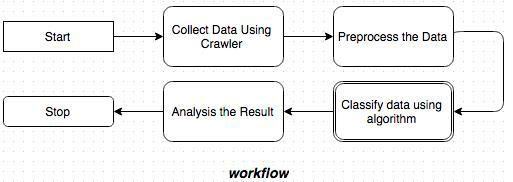
\includegraphics[scale=0.5]{images/fig-5.jpg}
\caption{Workflow}
\label{fig:x Workflow}
\end{figure}


\nomenclature{$\upsilon$}{Upsilon}
\nomenclature{$\epsilon$}{Epsilon}


\chapter{First and Second}
%\section{First and Second}
\section{Result Prediction based on First and Second Segment (Bat First)} 
As we have divided our total model into three segment and we actually consider first two segment for predicting the match outcome as we wanted to find out the final match result when match is in progress. We have taken total 91 match for making our model using multiple linear regression and we have merged all the attributes from those matches based on different segment. After analyzing those two segment our model has given 75\% accuracy. So, we can predict any match outcome when the match is in progress based on our model. As we did not take any attributes from the team who will bat second and considering the attribute which we got from first segment, our predicted model is quite good.

\begin{figure}[htbp]
\centering
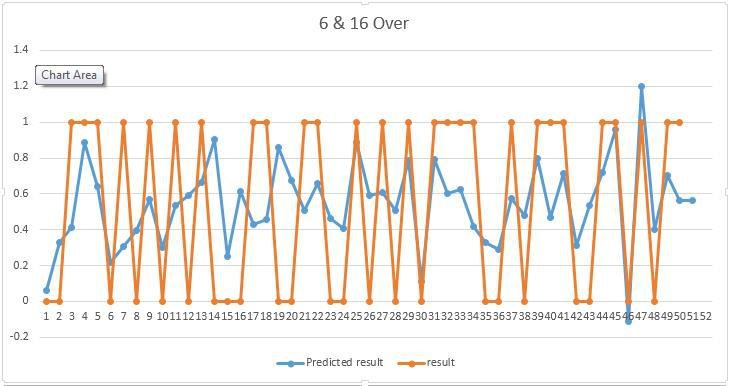
\includegraphics[scale=0.5]{images/fig-17.jpg}
\caption{First and Second Segment Prediction (Bat First)}
\label{fig:x First and Second Segment Prediction (Bat First)}
\end{figure}

From the figure above we can see the graph view of our model, here 0 means lost and 1 means win. So, if the predictive final value is less than 0.5 then the result would be consider as lose and if the predictive value is greater than 0.5 then it would be consider as win.

\textbf{Coefficient:} These are the coefficients values for all the attributes from Win prediction based on bat first.

\begin{table}[htbp]
\centering
\begin{tabular}{l | l}
Attributes & Coefficients\\
\hline
Intercept & 0.092219\\
Venue & 0.242112\\
M6ORN & 0.039573\\
M6OW & -0.12872\\
M16ORN & 0.05121\\
M16OW & -0.07214
\end{tabular}
\caption{First and Second Coefficient (Bat First)}
\label{tab:First and Second Coefficient (Bat First)}
\end{table}

\textbf{P-values:} These are the p values for all the at-tributes from Win prediction based on bat first.

\begin{table}[htbp]
\centering
\begin{tabular}{|l | r|}
\hline
Attributes & P-value\\
\hline
Intercept & 0.87596\\
\hline
Venue & 0.088577\\
\hline
M6ORN & 0.323375\\
\hline
M6OW & 0.084286\\
\hline
M16ORN & 0.246463\\
\hline
M16OW & 0.254117\\
\hline
\end{tabular}
\caption{First and Second Segment P-value (Bat First)}
\label{tab:First and Second Segment P-value (Bat First)}
\end{table}

\section{Result Prediction based on First and Second Segment (Bat Second)} 
While calculating for 2nd innings segments we get the run rate value from team batting first. Which makes a better impact on a prediction model and that time our model has given 85.5\% accuracy which is really good.

\begin{figure}[htbp]
\centering
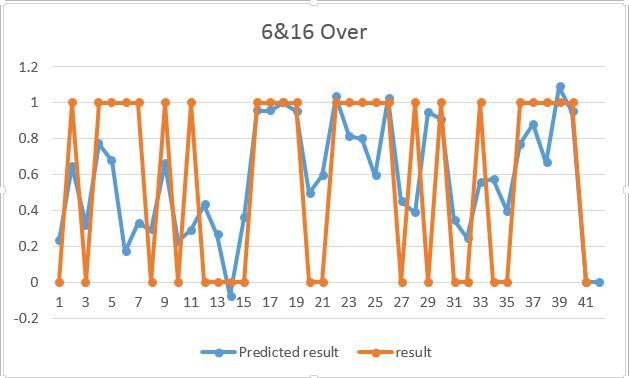
\includegraphics[scale=0.5]{images/fig-18.jpg}
\caption{First and Second Segment Run Prediction (Bat Second)}
\label{fig:x Frist and Second Segment Run Prediction (Bat Second)}
\end{figure}

\textbf{Coefficient:} These are the coefficients values for all the attributes from Win prediction based on bat second.
\vspace{3cm}

\begin{table}[htbp]
\centering
\begin{tabular}{|l | l|}
\hline
Attributes & Coefficients\\
\hline
Intercept & 2.282567\\
Venue & -0.04063\\
M6ORN & -0.02869\\
M6OW & -0.22694\\
M16ORN & -0.12705\\
M16OW & -0.10903\\
O6ORN & 0.008056\\
060W & 0.066748\\
O16ORN & 0.028731\\
O16OW & -0.0978\\
\hline
\end{tabular}
\caption{First and Second Segment Coefficient (Bat Second)}
\label{tab:First and Second Segment Coefficient (Bat Second)}
\end{table}

\textbf{P-values:} These are the p values for all the at-tributes from Win prediction based on bat second.

\setlength{\arrayrulewidth}{0.5mm}
\setlength{\tabcolsep}{12pt}
\renewcommand{\arraystretch}{1.5}

\begin{table}[ht]
\centering
\begin{tabular}{|l | l|}
\hline
\multicolumn{2}{| c |}{First and Second Segment P-value (Bat Second)} \\
\hline
Attributes & Coefficients\\
\hline
Intercept & 0.007165\\
Venue & 0.811504\\
M6ORN & 0.482433\\
M6OW & 0.019258\\
M16ORN & 0.112474\\
M16OW & 0.090761\\
O6ORN & 0.878555\\
060W & 0.429492\\
O16ORN & 0.633494\\
O16OW & 0.179298\\
\hline
\end{tabular}
\caption{First and Second Segment P-value (Bat Second)}
\label{tab:First and Second Segment P-value (Bat Second)}
\end{table}


\phantomsection
\printbibliography % Where the bibliography will be printed
\addcontentsline{toc}{chapter}{Bibliography}

% ********************************** Appendices ********************************
%\begin{appendices} % Using appendices environment for more functionality
\newpage
\phantomsection
\addcontentsline{toc}{chapter}{Appendix A How to install \LaTeX}
% ******************************* Thesis Appendix A ****************************
\chapter*{How to install \LaTeX} 

\section*{Windows OS}

\subsection*{TeXLive package - full version}
\begin{enumerate}
\item	Download the TeXLive ISO (2.2GB) from\\
\href{https://www.tug.org/texlive/}{https://www.tug.org/texlive/}
\item	Download WinCDEmu (if you don't have a virtual drive) from \\
\href{http://wincdemu.sysprogs.org/download/}
{http://wincdemu.sysprogs.org/download/}
\item	To install Windows CD Emulator follow the instructions at\\
\href{http://wincdemu.sysprogs.org/tutorials/install/}
{http://wincdemu.sysprogs.org/tutorials/install/}
\item	Right click the iso and mount it using the WinCDEmu as shown in \\
\href{http://wincdemu.sysprogs.org/tutorials/mount/}{
http://wincdemu.sysprogs.org/tutorials/mount/}
\item	Open your virtual drive and run setup.pl
\end{enumerate}

or

\subsection*{Basic MikTeX - \TeX~ distribution}
\begin{enumerate}
\item	Download Basic-MiK\TeX (32bit or 64bit) from\\
\href{http://miktex.org/download}{http://miktex.org/download}
\item	Run the installer 
\item	To add a new package go to Start >> All Programs >> MikTex >> Maintenance (Admin) and choose Package Manager
\item	Select or search for packages to install
\end{enumerate}

\subsection*{TexStudio - \TeX~ editor}
\begin{enumerate}
\item	Download TexStudio from\\
\href{http://texstudio.sourceforge.net/\#downloads}
{http://texstudio.sourceforge.net/\#downloads} 
\item	Run the installer
\end{enumerate}

\section*{Mac OS X}
\subsection*{MacTeX - \TeX~ distribution}
\begin{enumerate}
\item	Download the file from\\
\href{https://www.tug.org/mactex/}{https://www.tug.org/mactex/}
\item	Extract and double click to run the installer. It does the entire configuration, sit back and relax.
\end{enumerate}

\subsection*{TexStudio - \TeX~ editor}
\begin{enumerate}
\item	Download TexStudio from\\
\href{http://texstudio.sourceforge.net/\#downloads}
{http://texstudio.sourceforge.net/\#downloads} 
\item	Extract and Start
\end{enumerate}


\section*{Unix/Linux}
\subsection*{TeXLive - \TeX~ distribution}
\subsubsection*{Getting the distribution:}
\begin{enumerate}
\item	TexLive can be downloaded from\\
\href{http://www.tug.org/texlive/acquire-netinstall.html}
{http://www.tug.org/texlive/acquire-netinstall.html}.
\item	TexLive is provided by most operating system you can use (rpm,apt-get or yum) to get TexLive distributions
\end{enumerate}

\subsubsection*{Installation}
\begin{enumerate}
\item	Mount the ISO file in the mnt directory
\begin{verbatim}
mount -t iso9660 -o ro,loop,noauto /your/texlive####.iso /mnt
\end{verbatim}

\item	Install wget on your OS (use rpm, apt-get or yum install)
\item	Run the installer script install-tl.
\begin{verbatim}
	cd /your/download/directory
	./install-tl
\end{verbatim}
\item	Enter command `i' for installation

\item	Post-Installation configuration:\\
\href{http://www.tug.org/texlive/doc/texlive-en/texlive-en.html\#x1-320003.4.1}
{http://www.tug.org/texlive/doc/texlive-en/texlive-en.html\#x1-320003.4.1} 
\item	Set the path for the directory of TexLive binaries in your .bashrc file
\end{enumerate}

\subsubsection*{For 32bit OS}
For Bourne-compatible shells such as bash, and using Intel x86 GNU/Linux and a default directory setup as an example, the file to edit might be \begin{verbatim}
edit $~/.bashrc file and add following lines
PATH=/usr/local/texlive/2011/bin/i386-linux:$PATH; 
export PATH 
MANPATH=/usr/local/texlive/2011/texmf/doc/man:$MANPATH;
export MANPATH 
INFOPATH=/usr/local/texlive/2011/texmf/doc/info:$INFOPATH;
export INFOPATH
\end{verbatim}
\subsubsection*{For 64bit OS}
\begin{verbatim}
edit $~/.bashrc file and add following lines
PATH=/usr/local/texlive/2011/bin/x86_64-linux:$PATH;
export PATH 
MANPATH=/usr/local/texlive/2011/texmf/doc/man:$MANPATH;
export MANPATH 
INFOPATH=/usr/local/texlive/2011/texmf/doc/info:$INFOPATH;
export INFOPATH

\end{verbatim}



%\subsection{Installing directly using Linux packages} 
\subsubsection*{Fedora/RedHat/CentOS:}
\begin{verbatim} 
sudo yum install texlive 
sudo yum install psutils 
\end{verbatim}


\subsubsection*{SUSE:}
\begin{verbatim}
sudo zypper install texlive
\end{verbatim}


\subsubsection*{Debian/Ubuntu:}
\begin{verbatim} 
sudo apt-get install texlive texlive-latex-extra 
sudo apt-get install psutils
\end{verbatim}


\newpage
\phantomsection
\addcontentsline{toc}{chapter}{Appendix B Overleaf: GitHub for \LaTeX\ projects}
% ******************************* Thesis Appendix B ********************************

\chapter*{Overleaf: GitHub for \LaTeX\ projects }

This Project was developed using Overleaf(\url{https://www.overleaf.com/}), an online \LaTeX\ editor that allows real-time collaboration and online compiling of projects to PDF format. In comparison to other \LaTeX\ editors, Overleaf is a server-based application, which is accessed through a web browser.




%\end{appendices}

\end{document}